\section{Nozioni di Base}

\subsection{Relazioni Binarie}
Riportiamo la definizione di \emph{relazione binaria} su uno o due insiemi, che sarà utile per definire formalmente il concetto di \emph{grafo}, fondamentale all'interno di questo elaborato.
\begin{definition}
    Chiameremo \emph{relazione binaria} su $A,B$ qualsiasi sottoinsieme del prodotto cartesiano $A \times B$.\\
    Chiameremo \emph{relazione binaria} su $A$ qualsiasi sottoinsieme del prodotto cartesiano $A \times A$.\\
	Diremo che $u,v$ sono \emph{in relazione} rispetto a $R$ se $(u,v) \in R$. In questo caso potremo usare la notazione $u R v$.
\end{definition}
Alcune relazioni binarie mostrano proprietà fondamentali, che presentiamo nella definizione seguente:
\begin{definition}
    Sia $R$ una relazione binaria su $A$. Diremo che $R$ è
    \begin{itemize}
        \item \emph{riflessiva} se $\forall x \in A, x R x$;
        \item \emph{simmetrica} se $x R y \implies y R x \,\,(x,y \in A)$
        \item \emph{transitiva} se $(x R y \land y R z) \implies x R z \,\,(x,y,z \in A)$
    \end{itemize}
\end{definition}
\begin{example}
    La relazione $\leq$ sui naturali è riflessiva e transitiva, ma non simmetrica.\\
    La relazione $=$ ($a = b \iff $``$a,b$ sono lo stesso numero'') sui naturali è simmetrica, riflessiva e transitiva.
\end{example}
\begin{definition}
    Una relazione binaria riflessiva, simmetrica e transitiva si dice \emph{relazione di equivalenza}.\\
    Una relazione di equivalenza divide un insieme in \emph{classi di equivalenza} all'interno delle quali tutte le coppie di elementi sono in relazione.
\end{definition}
A partire da una relazione binaria $R$ possiamo costruire relazioni binarie che contengono $R$, e che mostrano una o più delle proprietà presentate sopra, le cosiddette \emph{chiusure}.
Ogni chiusura è costituita dall'unione della relazione iniziale e di un insieme di coppie costruito con un criterio differente a seconda del tipo di chiusura, che fornisce la proprietà desiderata.
\begin{definition}
	Sia $R$ una relazione binaria su $A$.
    Definiamo le seguenti chiusure:
    \begin{itemize}
        \item \emph{riflessiva}: $R_r = R \cup \{(x,x) \,\, \forall x \in A\}$
        \item \emph{simmetrica}: $R_s = R \cup \{(y,x) \,\, \forall x,y : (x,y) \in R\}$
        \item \emph{transitiva}: $R_t = R \cup \{(x,z) \,\, \forall x,z : \exists y : (x,y) \in R \land (y,z) \in R\}$
    \end{itemize}
\end{definition}
\begin{example}
    La chiusura riflessiva della relazione $<$ (minore stretto) è la relazione $\leq$.\\
    La chiusura transitiva della relazione $a R b \iff $``$a$ è più piccolo di $b$'' è la relazione $<$.
\end{example}

\subsection{Grafi}
Con queste premesse possiamo definire un \emph{grafo} come segue:
\begin{definition}
    Sia $V$ un insieme finito non vuoto. Sia $\to$ una relazione binaria su $V$.\\
    Chiameremo \emph{grafo diretto} o \emph{grafo orientato} la coppia $G = (V, \to)$.\\
    In questo caso
    \begin{itemize}
        \item $V$ è l'insieme dei \emph{nodi} o \emph{vertici};
        \item $\to$ è la relazione binaria che mette in relazione alcuni dei nodi di $G$
    \end{itemize}
\end{definition}
\begin{example}
    \begin{figure}[b]
        \centering
        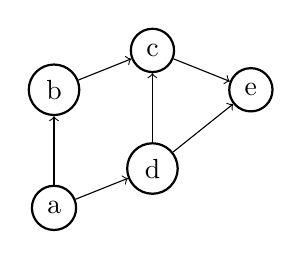
\begin{tikzpicture}[scale=0.5]
            \begin{scope}[every node/.style={circle,thick,draw}]
                \node (a) at (0,0) {a};
                \node (b) at (0,3) {b};
                \node (c) at (2.5,4) {c};
                \node (d) at (2.5,1) {d};
                \node (e) at (5,3) {e};
            \end{scope}

            \begin{scope}
                \path [->] (a) edge node {} (b);
                \path [->] (b) edge node {} (c);
                \path [->] (a) edge node {} (d);
                \path [->] (d) edge node {} (c);
                \path [->] (d) edge node {} (e);
                \path [->] (c) edge node {} (e);
            \end{scope}
            \end{tikzpicture}
        \caption{Rappresentazione grafica di un grafo}
        \label{fig:graph}
    \end{figure}
    Il grafo di Figura \ref*{fig:graph} è descritto dalla coppia
    \begin{itemize}
        \item $N = \{a,b,c,d,e\}$
        \item $\to \,\,= \{(a,b), (a,d), (b,c), (d,c), (c,e), (d,e)\}$
    \end{itemize}
\end{example}
Nel seguito utilizzeremo ampiamente la seguente terminologia:
\begin{definition}
    Sia $G = (V,\to)$ un grafo. Diremo che un nodo $u \in V$ è una \emph{foglia} se $\nexists v \in V : u \to v$. Diremo che $u$ è parente di $v$ e che $v$ è figlio di $u$ se $u \to v$.
\end{definition}
Un grafo è quindi un insieme di elementi (i \emph{nodi}) accoppiato con un insieme di relazioni tra questi elementi (gli \emph{archi} o \emph{rami}).\\
\accente naturale associare questo concetto all'idea di percorso: ogni grafo è definito da un insieme di nodi ed un insieme di \emph{cammini} che consentono di spostarsi da un nodo ad un altro.\\
La seguente definizione sorge in modo spontaneo da questo punto di vista:
\begin{definition}
    Sia $G = (V, \to)$ un grafo. Siano $u,v \in V$. Diremo che $v$ \emph{è raggiungibile da} $u$, o in alternativa \emph{esiste un cammino da} $u$ \emph{a} $v$, o ancora $u \to_t v$ (la $t$ in pedice sta per ``\emph{transitivo}''), se
    $\exists x_n \subset V$ (una sequenza finita di nodi) di lunghezza $K : x_K = v, x_0 = u, x_n \to x_{n+1}$.
\end{definition}
L'esistenza di un cammino tra nodi fornisce un criterio immediato per partizionare un grafo in gruppi di nodi. Diamo innanzitutto la seguente definizione:
\begin{definition}
    Diremo che un grafo $(V,\to)$ è \emph{fortemente connesso} se $\forall v_1, v_2 \in V, v_1 \to_t v_2$.\\
    Le \emph{componenti fortemente connesse} (\emph{CFC}) di un grafo $(V,\to)$ sono le classi di equivalenza della relazione $\to_t$ \cite[Appendice B]{clrs}. In altre parole, i nodi contenuti in una stessa componente fortemente connessa sono mutuamente raggiungibili.
\end{definition}
\begin{example}
    \begin{figure}[b]
        \centering
        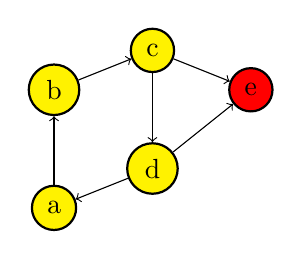
\begin{tikzpicture}[scale=0.5]
            \begin{scope}[every node/.style={circle,thick,draw}]
                \node (a)[fill=yellow] at (0,0) {a};
                \node (b)[fill=yellow] at (0,3) {b};
                \node (c)[fill=yellow] at (2.5,4) {c};
                \node (d)[fill=yellow] at (2.5,1) {d};
                \node (e)[fill=red] at (5,3) {e};
            \end{scope}

            \begin{scope}
                \path [->] (a) edge node {} (b);
                \path [->] (b) edge node {} (c);
                \path [->] (d) edge node {} (a);
                \path [->] (c) edge node {} (d);
                \path [->] (d) edge node {} (e);
                \path [->] (c) edge node {} (e);
            \end{scope}
            \end{tikzpicture}
        \caption{CFC di un grafo}
        \label{fig:graph_cfc_1}
    \end{figure}
    Nel grafo di Figura \ref*{fig:graph_cfc_1} le CFC sono state evidenziate con colori diversi: $\{a,b,c,d\}, \{e\}$.
\end{example}
Il partizionamento in CFC è definito come segue:
\begin{definition}
    Sia $G = (V, \to)$ un grafo. Chiameremo \emph{grafo delle componenti fortemente connesse (CFC) di} $G$ il grafo $G^{CFC} = (V^{CFC}, \to^{CFC})$ con
    \begin{itemize}
        \item $V^{CFC} = \{C : \,$``$C$ è una classe di equivalenza per $\to_t$ su $V$''$\}$
        \item $\to^{CFC} = \{(A,B) \in V^{CFC} \times V^{CFC} : A \neq B, \exists m \in A, n \in B : m \to n\}$
    \end{itemize}
\end{definition}
Riportiamo la seguente proprietà immediata:
\begin{proposition}
    Sia $G^{CFC}$ il grafo delle CFC di un grafo $G$ generico. Allora $G^{CFC}$ è aciclico.
\end{proposition}
\begin{proof2}
    Suppongo per assurdo che in $G^{CFC}$ esista un ciclo. Allora tutti i nodi di $V^{CFC}$ facenti parte del ciclo sono mutuamente raggiungibili (percorrendo il ciclo). Quindi tutti i nodi fanno parte della stessa CFC, ma questo è assurdo.
\end{proof2}
\begin{example}
    \begin{figure}[t]
        \centering
        \begin{subfigure}{.45\textwidth}
          \centering
          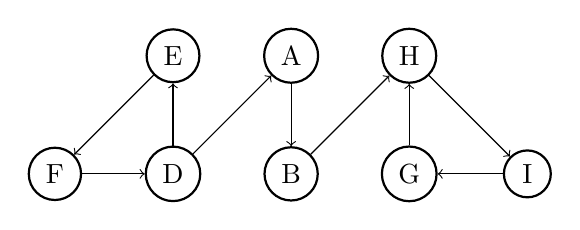
\begin{tikzpicture}[scale=0.5]
            \begin{scope}[every node/.style={circle,thick,draw}]
                \node (A) at (0,3) {A};
                \node (B) at (0,0) {B};

                \node (D) at (-3,0) {D};
                \node (E) at (-3,3) {E};
                \node (F) at (-6,0) {F};

                \node (G) at (3,0) {G};
                \node (H) at (3,3) {H};
                \node (I) at (6,0) {I};
            \end{scope}

            \begin{scope}
                \path [->] (A) edge node {} (B);

                \path [->] (E) edge node {} (F);
                \path [->] (F) edge node {} (D);
                \path [->] (D) edge node {} (E);

                \path [->] (G) edge node {} (H);
                \path [->] (H) edge node {} (I);
                \path [->] (I) edge node {} (G);

                \path [->] (D) edge node {} (A);
                \path [->] (B) edge node {} (H);
            \end{scope}
            \end{tikzpicture}
          \caption{Un grafo}
        \end{subfigure}
        \hfill
        \begin{subfigure}{.45\textwidth}
          \centering
          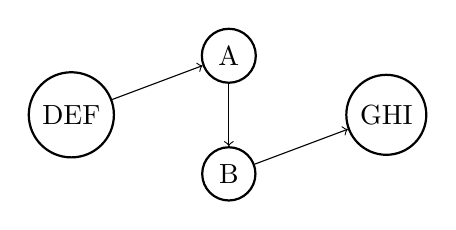
\begin{tikzpicture}[scale=0.5]
            \begin{scope}[every node/.style={circle,thick,draw}]
                \node (A) at (0,3) {A};
                \node (B) at (0,0) {B};

                \node (DEF) at (-4,1.5) {DEF};

                \node (GHI) at (4,1.5) {GHI};
            \end{scope}
                \path [->] (A) edge node {} (B);
                \path [->] (DEF) edge node {} (A);
                \path [->] (B) edge node {} (GHI);
            \begin{scope}

            \end{scope}
            \end{tikzpicture}
          \caption{Grafo delle CFC}
        \end{subfigure}
        \caption{Un grafo ed il corrispondente grafo delle CFC}
        \label{fig:graph_cfc_2}
    \end{figure}
    La Figura \ref*{fig:graph_cfc_2}.a rappresenta un grafo generico, la Figura \ref*{fig:graph_cfc_2}.b rappresenta il suo grafo delle componenti fortemente connesse associato.
\end{example}

\subsection{Insiemi}
\subsubsection{Cenni di teoria degli insiemi}
In generale ammettiamo che un insieme possa contenere altri insiemi. Questa concessione diventa problematica nel caso in cui tra i membri di un insieme $A$ risulti lo stesso insieme $A$, o un insieme contenente l'insieme $A$. Diamo quindi la seguente definizione:
\begin{definition}
    Diremo che un insieme $A$ è \emph{ben-fondato} se $\forall B \in A : $ ``B è un insieme'' si ha $A \not\subset B$. Altrimenti diremo che $A$ è \emph{non-ben-fondato}.
\end{definition}
\begin{example}
    L'insieme $\Omega = \{\Omega\}$ è non-ben-fondato. L'insieme $A = \{1,2,3\}$ è ben-fondato.
\end{example}
% TODO: definisci insieme ereditariamente finito (si può costruire a partire dall'insieme vuoto utilizzando solamente il costruttore {} vedi ZFC) e insime non-ben-fondato prima di usare i grafi per rappresentare gli insiemi

\subsubsection{Rappresentazione di insiemi tramite grafi}
\label{sec:graphs_sets}
In alcuni casi risulta conveniente fornire un'in\-ter\-pre\-ta\-zio\-ne insiemistica della nozione di grafo vista sopra. Introduciamo innanzitutto una nozione fondamentale:
\begin{definition}
    Sia $G = (V, \to)$ un grafo orientato. Sia $u \in V : \forall v \in V, u \to_t v$, cioè ogni nodo di $G$ è raggiungibile da $u$. Allora la terna $(V, \to, u)$ si dice \emph{accessible pointed graph}, o \emph{APG}.
\end{definition}
Per pervenire allo scopo di rappresentare un insieme tramite un grafo è necessario definire un processo denominato \emph{decorazione}:
\begin{definition}
    Chiameremo \emph{decorazione} di un APG l'assegnazione di un insieme ad ogni suo nodo.
\end{definition}
Associando la relazione di raggiungibilità $\to$ alla relazione di appartenenza $\in$ abbiamo tutto il necessario per la rappresentazione di insiemi:
\begin{definition}
    Chiameremo \emph{immagine} (o \emph{picture} in \cite{aczel}) di un insieme $A$ la coppia di un APG $(G,v)$ con una decorazione in cui a $v$ è associato $A$.
\end{definition}
Ad un APG aciclico è possibile associare un'unica decorazione. Questo risultato tuttavia non può essere dimostrato nel caso di un APG contenente almeno un ciclo. Per questo motivo in \cite{aczel} viene dato il seguente assioma:
\begin{axiom}[AFA, Anti-Foundation-Axiom]
    Ogni APG possiede un'unica decorazione.
\end{axiom}
L'assioma AFA ha un'ovvia conseguenza:
\begin{corollary}
    Ogni APG è immagine di un unico insieme.
\end{corollary}
\begin{example}
    \begin{figure}[b]
        \centering
        \begin{subfigure}{.25\textwidth}
          \centering
          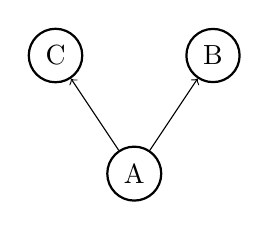
\begin{tikzpicture}[scale=0.5]
            \begin{scope}[every node/.style={circle,thick,draw}]
                \node (A) at (0,0) {A};
                \node (B) at (2,3) {B};
                \node (C) at (-2,3) {C};
            \end{scope}

            \begin{scope}
                \path [->] (A) edge node {} (B);
                \path [->] (A) edge node {} (C);
            \end{scope}
            \end{tikzpicture}
          \captionsetup{labelformat=empty}
          \caption{$\{\emptyset\}$}
        \end{subfigure}
        \begin{subfigure}{.15\textwidth}
            \centering
            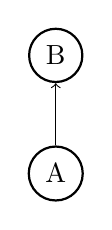
\begin{tikzpicture}[scale=0.5]
              \begin{scope}[every node/.style={circle,thick,draw}]
                  \node (A) at (0,0) {A};
                  \node (B) at (0,3) {B};
              \end{scope}

              \begin{scope}
                  \path [->] (A) edge node {} (B);
              \end{scope}
              \end{tikzpicture}
            \captionsetup{labelformat=empty}
            \caption{$\{\emptyset\}$}
          \end{subfigure}
        \begin{subfigure}{.15\textwidth}
          \centering
          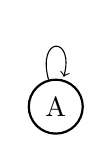
\begin{tikzpicture}[scale=0.5]
            \begin{scope}[every node/.style={circle,thick,draw}]
                \node (A) at (0,-1) {A};
            \end{scope}

            \begin{scope}
                \path [->] (A) edge [loop above] node {} (A);
            \end{scope}
            \end{tikzpicture}
          \captionsetup{labelformat=empty}
          \caption{$A = \{A\}$}
        \end{subfigure}
        \begin{subfigure}{.25\textwidth}
            \centering
            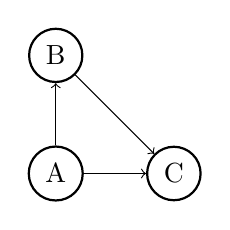
\begin{tikzpicture}[scale=0.5]
              \begin{scope}[every node/.style={circle,thick,draw}]
                  \node (A) at (0,0) {A};
                  \node (B) at (0,3) {B};
                  \node (C) at (3,0) {C};
              \end{scope}

              \begin{scope}
                  \path [->] (A) edge node {} (B);
                  \path [->] (B) edge node {} (C);
                  \path [->] (A) edge node {} (C);
              \end{scope}
              \end{tikzpicture}
            \captionsetup{labelformat=empty}
            \caption{$\{\emptyset, \{\emptyset\}\}$}
          \end{subfigure}

        \caption{Rappresentazione di insiemi tramite grafi}
        \label{fig:graph_set}
    \end{figure}
    In Figura \ref*{fig:graph_set} sono rappresentati alcuni insiemi sotto forma di APG.
\end{example}
In \cite{aczel} viene fornita una formulazione alternativa dell'assioma AFA, data dalla congiunzione dei seguenti assiomi:
\begin{axiom}(AFA1)
    Ogni grafo ha almeno una decorazione.
\end{axiom}
\begin{axiom}(AFA2)
    Ogni grafo ha al più una decorazione.
\end{axiom}
Chiaramente le due formulazioni sono equivalenti. Consideriamo adesso la seguente relazione binaria su insiemi:
\begin{gather*}
    a \equiv b \iff \text{``esiste un APG che è immagine di entrambi''}
\end{gather*}
\begin{proposition}
    AFA2 e $(a \equiv b \implies a = b)$ sono equivalenti.
\end{proposition}
\begin{proof2}
    Supponendo valido AFA2, la decorazione di un APG (immagine di $a,b$) è unica. Quindi $a,b$ devono necessariamente essere lo stesso insieme.\\
    Supponendo $(a \equiv b \implies a = b)$, se per assurdo esistesse un APG avente più di una decorazione, i due insiemi rappresentati dalle coppie (APG, ``Decorazione \#1''), (APG, ``Decorazione \#2'') sono uguali.
\end{proof2}
La formulazione alternativa di AFA sarà utile nel seguito, in quanto consente di collegare il concetto di \emph{bisimulazione} con la teoria degli insiemi.

\subsection{Bisimulazione}
\begin{definition}
    Siano $G_1 = (V_1,\to_1), G_2 = (V_2,\to_2)$ due grafi. Diremo che una relazione binaria $R: V_1 \times V_2$ è una \emph{bisimulazione} su $G_1, G_2$ se $\forall a \in V_1, b \in V_2$ valgono congiuntamente le seguenti proprietà:
    \begin{itemize}
        \item $a R b, a \to_1 a' \implies \exists b' \in V_2 : (a' R b' \land b \to_2 b')$
        \item $a R b, b \to_2 b' \implies \exists a' \in V_1 : (a' R b' \land a \to_1 a')$
    \end{itemize}
    Possiamo definire in modo analogo una bisimulazione su un unico grafo $G$, ponendo $G_1 = G_2 = G$.
\end{definition}
Definiamo un'importante caratteristica di una coppia qualsiasi di grafi, che verrà sfruttata ampiamente nel seguito
\begin{definition}
    Siano $G_1 = (V_1,\to_1), G_2 = (V_2,\to_2)$ due grafi. Diremo che sono \emph{bisimili} se $\exists R: V_1 \times V_2 : R$ è una bisimulazione su $G_1, G_2$.\\
    Diremo che due APG $(G_1, v_1), (G_2, v_2)$ sono \emph{bisimili} se $G_1, G_2$ sono bisimili e vale $v_1 R v_2$ per almeno una bisimulazione su $G_1, G_2$.
\end{definition}
\begin{observation}
    Una bisimulazione può non essere riflessiva, simmetrica, nè transitiva.
\end{observation}
\begin{example}
    La relazione $a R b \iff$ ``$a,b$ sono lo stesso nodo'' su un grafo qualsiasi è una bisimulazione riflessiva, simmetrica e transitiva.
\end{example}
Dalla definizione di bisimulazione possiamo dedurre una proprietà interessante di una qualsiasi sua chiusura:
\begin{theorem}
    Sia $b$ una bisimulazione sul grafo $G$. La sua chiusura riflessiva, simmetrica o transitiva è ancora una bisimulazione su $G$.
\end{theorem}
\begin{proof2}
    Consideriamo separatamente le tre relazioni $b_r, b_s, b_t$, rispettivamente la chiusura riflessiva, simmetrica e transitiva:
    \begin{itemize}
        \item[$b_r$] Per definizione $b \subset b_r$, quindi è sufficiente dimostrare che $b_r$ è una bisimulazione quando gli argomenti $u,v \in N$ non sono distinti.\\
        Sia $u \in N$. Chiaramente per definizione di $b_r$ si ha $u b_r u$. Se $\exists u' \in N : u \to u'$ allora (sempre per definizione di $b_r$) si ha $u' b_r u'$.
        \item[$b_s$] Per definizione $b \subset b_s$, quindi è sufficiente dimostrare che $b_s$ è una bisimulazione quando per gli argomenti $u,v \in N$ si ha $u b v$ ma non $v b u$.\\
        Sia $(u,v) \in N \times N$. Allora
        \begin{center}
            $u b_s v \implies u b v \lor v b u$
        \end{center}
        Suppongo ad esempio che $v b u$.
        \begin{align*}
            &\implies \forall v' \in N : (v \to v') \,\,\exists u' \in N : (u \to u' \land v' bu')\\
            &\implies u' b_s v'
        \end{align*}
        e
        \begin{align*}
            &\implies \forall u' \in N : (u \to u') \,\,\exists v' \in N : (v \to v' \land v' bu')\\
            &\implies u' b_s v'
        \end{align*}
        cioè sono dimostrate le due condizioni caratteristiche della bisimulazione.\\
        La dimostrazione è analoga se $u b v$.
        \item[$b_t$] Per definizione $b \subset b_t$, quindi è sufficiente dimostrare che $b_t$ è una bisimulazione quando per gli argomenti $u,v,z \in N$ si ha $u b v$, $v b z$ ma non $u b z$.\\
        Sia $(u,v,z) \in N \times N \times N$ con questa proprietà. Allora $\forall u' \in N : u \to u' \implies \exists v' \in N : v \to v' \land u' b v'$. Inoltre $\exists z' : z \to z' \land v' b z'$.\\
        Riordinando si ha $u' b v', v' b z'$. Allora per definizione di $b_t, \, u' b_t z'$.\\
        In modo speculare si ottiene la seconda condizione caratteristica della bisimulazione.
    \end{itemize}
\end{proof2}
Da questa proposizione si deduce il seguente corollario, che risulta dall'applicazione iterativa delle tre chiusure viste in precedenza:
\begin{corollary}
    Ad ogni bisimulazione $b$ è possibile associare una bisimulazione $\widetilde{b} : b \subset \widetilde{b} \,\,\land\,\, \widetilde{b}$ è una relazione di equivalenza.
    \label{cor:bisimulation_eqrel}
\end{corollary}
Concludiamo la sezione relativa ai risultati generali sulla bisimulazione con la seguente proposizione, che sarà utile nel seguito:
\begin{proposition}
    Siano $b_1, b_2$ due bisimulazioni su $G_1, G_2$. Allora $b = b_1 \cup b_2$ è ancora una bisimulazione.
    \label{obs:bisimulation_union}
\end{proposition}
\begin{proof2}
    Siano $u,v : u b v$. Sia $u' : u \to u'$. Allora deve essere $u b_1 v \lor u b_2 v$. Ma quindi $\exists v' : (v \to v' \land u' b_{1|2} v')$.
\end{proof2}

\subsubsection{Bisimulazione massima}
\label{sec:bisi_max}
Definiamo ora il concetto di \emph{bisimulazione massima}, che gioca un ruolo chiave nella risoluzione dei problemi considerati in questo elaborato.
\begin{definition}
    Diremo che una bisimulazione $b_M$ su $G_1, G_2$ è \emph{massima} se $\forall b : "b$ è una bisimulazione su $G_1, G_2$" si ha $u b v \implies u b_M v \,\,\,\forall a \in N_1, b \in N_2$.
\end{definition}
Naturalmente la bisimulazione massima dipende dai due grafi presi in esame. Possiamo dedurre alcune caratteristiche in modo molto semplice:
\begin{proposition}
    Valgono le seguenti proprietà:
    \begin{enumerate}
        \item La bisimulazione massima su due grafi $G_1,G_2$ è unica
        \item La bisimulazione massima è una relazione di equivalenza
    \end{enumerate}
\end{proposition}
\begin{proof2}
    Le proprietà seguono banalmente dal Corollario \ref*{cor:bisimulation_eqrel} e dall'Osservazione \ref*{obs:bisimulation_union}.
    \begin{enumerate}
        \item Suppongo per assurdo che esistano due bisimulazioni massime $b_{M_1}, b_{M_2}$. La loro unione è ancora una bisimulazione, che è "più massima" delle supposte bisimulazioni massime.
        \item Se per assurdo la bisimulazione massima non fosse una relazione di equivalenza, potremmo considerare la sua chiusura riflessiva, simmetrica e transitiva, che sarebbe "più massima" ed anche una relazione di equivalenza.
    \end{enumerate}
\end{proof2}
Naturalmente il concetto di \emph{bisimulazione massima} può essere definito anche su unico grafo $G$. Questo caso si rivelerà di grande interesse nel seguito. Per
ora dimostriamo il seguente risultato:
\begin{theorem}
    Sia $G$ un grafo (finito). Allora $\exists b_M$ la bisimulazione massima su $G$.
\end{theorem}
\begin{proof2}
    Può esistere solamente un numero finito di relazioni binarie su $G$, e questo numero fornisce un limite superiore al numero massimo di bisimulazioni su $G$.
    Allora possiamo considerare l'unione di questo numero finito di bisimulazioni, che sarà chiaramente la bisimulazione massima.
\end{proof2}

\subsubsection{Interpretazione insiemistica della bisimulazione}
Il seguente teorema è la prova che la bisimulazione può essere utilizzata per verificare l'uguaglianza tra insiemi rappresentati da due APG differenti:
\begin{theorem}
    Due APG sono bisimili $\iff$ rappresentano lo stesso insieme.
    \label{theo:bisi_iff_eqsets}
\end{theorem}
\begin{proof2}
    Da dimostrare...
\end{proof2}
Tenendo conto di quanto affermato nella sezione \ref*{sec:graphs_sets}, il Teorema \ref*{theo:bisi_iff_eqsets} dimostra che la bisimulazione può sostituire la
relazione di uguaglianza tra insiemi quando questi sono rappresentati da degli APG \cite{dovier}.\\
Dopo questa considerazone, risulta naturale definire il seguente concetto:
\begin{definition}
    Sia $b$ una bisimulazione su $G$ che sia anche una relazione di equivalenza. Definiamo un nuovo grafo $G_b = (N_b, \to_b)$ come in \cite{gentilini}, che chiameremo \emph{contrazione rispetto alla bisimulazione} $b$ \emph{di} $G$:
    \begin{itemize}
        \item $N_b = \{A = \{m \in N : \forall n \in A, m b n\}\}$
        \item $[m]_b \to_b [n]_b \iff \exists c \in [n]_b : m \to c$
    \end{itemize}
    Risulta conveniente definire la \emph{classe del nodo} $a$ rispetto alla bisimulazione $b$, con la notazione $[a]_b$ come il nodo di $N_b$ a cui appartiene il nodo $a$.
    \label{def:bisi_contraction}
\end{definition}
La Definizione \ref*{def:bisi_contraction} è di fondamentale importanza per la seguente osservazione:
\begin{proposition}
    Sia $G$ un grafo, e sia $G_b$ come nella Definizione \ref*{def:bisi_contraction}, per una bisimulazione $b$ qualsiasi. Allora $G, G_b$ sono bisimili.
    \label{prop:bisi_cont_bisi}
\end{proposition}
\begin{proof2}
    Sia $\equiv \,\,\subset N \times N_b$ la relazione binaria definita come segue:
    \begin{gather*}
        m \equiv M \iff M = [m]_b
    \end{gather*}
    Vogliamo dimostrare che tale relazione è una bisimulazione su i grafi $G, G_b$.\\
    Supponiamo che $x \equiv X$, e che $x \to y$ per qualche $y \in N$. Chiamiamo $Y \coloneqq [y]_b$. Allora, per la Definizione \ref*{def:bisi_contraction}, si ha $X \to Y$. Inoltre vale banalmente $y \equiv Y$.\\
    Per dimostrare la seconda condizione caratteristica della bisimulazione, supponiamo che $x \equiv X$, e che $X \to Y$ per qualche $Y \in N_b$. Sempre per la Definizione \ref*{def:bisi_contraction} deve esistere un $y \in Y : (y \equiv Y \land x \to y)$.
\end{proof2}
La Proposizione \ref*{prop:bisi_cont_bisi} ha una conseguenza ovvia, che risulta evidente per il Teorema \ref*{theo:bisi_iff_eqsets}:
\begin{corollary}
    Sia $b$ una bisimulazione che sia anche una relazione di equivalenza. Allora l'APG $(G, v)$ e l'APG $(G_b, [v]_b)$ rappresentano lo stesso insieme.
\end{corollary}
Quindi risulta naturale sfruttare le proprietà della bisimulazione per minimizzare la rappresentazione di insiemi, considerando che è sufficiente una bisimulazione sulla rappresentazione iniziale per ottenere una rappresentazione equivalente. Definiamo una relazione d'ordine sulle rappresentazioni:
\begin{definition}
    Diremo che la rappresentazione $(G_a, v_a)$ di un insieme è \emph{minore} della rappresentazione equivalente $(G_b, v_b)$ se $\#N_a < \#N_b$.\\
    Diremo che una rappresentazione è \emph{minima} se non esiste un'altra rappresentazione minore.
\end{definition}
\begin{observation}
    La \emph{contrazione per bisimulazione} di un grafo ha sempre un numero di nodi minore o uguale di quello del grafo iniziale.
\end{observation}
Concludiamo la sezione con il seguente risultato, che stabilisce in modo univoco la bisimulazione prescelta per minimizzare la rappresentazione di un dato insieme:
\begin{theorem}
    Sia $(G,v)$ un APG rappresentante un insieme. Sia $b_M$ la bisimulazione massima su $(G,v)$. Allora la contrazione per bisimulazione indotta da $b_M$ su $(G,v)$ fornisce la rappresentazione minima dell'insieme.
\end{theorem}
\begin{proof2}
    Suppongo per assurdo che esista una bisimulazione $b_N$ su $(G,v)$ che fornisce una contrazione avente un numero di nodi strettamente inferiore alla contrazione indotta da $b_M$. Ma questo implica che esistono almeno due nodi di $G$ che sono in relazione secondo $b_N$ e non secondo $b_M$. Chiaramente questa deduzione è in contrasto con il fatto che $b_M$ è la bisimulazione massima.\\\\
    Suppongo per assurdo che, dopo la contrazione indotta da $b_M$, sia possibile trovare una nuova bisimulazione $b_O$ su $(G_{b_M}, [v]_{b_M})$ che induca una contrazione avente un numero di nodi strettamente inferiore a quello di $(G_{b_M}, [v]_{b_M})$. Chiaramente $b_O \subset N_{b_M} \times N_{b_M}$.\\
    Definisco una nuova bisimulazione $b_{\widetilde{M}} \subset N \times N$ tale che
    \begin{gather*}
        x b_{\widetilde{M}} y \iff (x b_M y \lor [x]_{b_M} b_O [y]_{b_M})
    \end{gather*}
    Per definizione di bisimulazione massima bisogna avere $b_{\widetilde{M}} \subset b_M$, quindi non è possibile che la contrazione indotta da $b_O$ sia una rappresentazione minore di quella indotta da $b_M$.
\end{proof2}
